\documentclass{article}

% packages
\usepackage{amsmath} % math
\usepackage{bm}
\usepackage{graphicx} % graph
\usepackage{float}
\usepackage{hyperref} % hyper-reference
\usepackage{indentfirst}  % indent in the first paragraph of a section

% settings
\usepackage{geometry}
\geometry{left=2.5cm,right=2.5cm,top=3.5cm,bottom=3.5cm}
\linespread{1.5}

\title{Consumer Quality Search and Platform Algorithm Design: A Structural Apporach}
\author{
Guo Zhang
\thanks{WISE, Xiamen University. Email: zhangguo@stu.xmu.edu.cn. 
All codes can be found here: \url{https://github.com/xmucpp/online_quality_search/blob/master/consumer_quality_search.ipynb}. 
This version will be reorganized and resubmitted to GitHub in the follow months. 
You can always find the new version from here: \url{https://github.com/Guo-Zhang/MyPapers/tree/master/online_quality_search}.}
}
\date{This Version: \today}


\begin{document}
\maketitle

\begin{abstract}
The improvement of algorithm design and mechanism design is one of the
most important reasons for the development of online platforms. 
This paper extends the model proposed by Levin et.al.(2014) to describe
consumer search on prices and qualities, sellers pricing and market equilibrium on the environment of platform ranking algorithms with consideration set approach. Then the optimal algorithm parameters are found to maximize the consumer welfare with estimates from sample data collected by China's Prices Project. 
\end{abstract}

\section{Introduction}

% Motivation and theme
The improvement of algorithm design and mechanism design is one of the
most important reasons for the development of online platforms. A tiny
improvement can worth millions of dollars for massive platforms. Studies
by academics and industries at present crowd on describing and
predicting, and rare researches until now work on the underlying
processes, which is concerned by both economists and executives.

A lot of economic studies have crowded on the organization given the design of online platforms. However, the underlying processes that makes platform algorithms work have not been clarified well. To improve the understanding of consumer online search processes to guide platform algorithm design, this paper is going to develop the work of Levin et.al.(2014), studying the online consumer search on product price and product quality, to discuss methods of improving platform ranking algorithms. 

% Summary
In this paper, the economics of online platform algorithms will be discussed beforehand in Section 2. Platforms gather buyers and sellers in the same market place to exchange products, services and information, reducing transaction costs and search costs for all users. However, the search costs still exist, so the platforms design a lot of mechanism and algorithms to overcome search and matching problems for users, such as ranking algorithms and recommender systems. This paper takes the product ranking algorithms as an example. The ranking algorithms allocate each relevant item a sampling weight, and the item with higher weights will be ranked to the tops with higher probabilities. The product ranking algorithms are very complicated in practice, influenced by indicators of products and their shops. To model the consumer search processes, the consideration set approach is applied in this paper. Consideration set is defined as the subset of products or brands considered when consumers make purchase decisions.  Sellers should consider the algorithms when making price decisions. However, sellers can also manipulate their signaled information to gain market power and more profits. 

% √
A structural model will be built, estimated and applied in the following sections. A model will be proposed to describe consumer search and choice, seller pricing and market equilibrium on the environment of platform ranking algorithms. Model parameters will be estimated in a single-product market with vertical differentation, including parameters of consumer utility, parameters of sampling weights by platform ranking algorithms and marginal costs of sellers. The estimates will be applied to find the optimal algorithm parameters which maximize the consumer welfare in the market.  

The model of consumer search and seller pricing in the environment of platform ranking algorithms will be described in Section 3. The platform ranking algorithm allocates each product with a sampling weight, and the products with higher sampling weights will be selected with higher probability when the ranking algorithm samples a product from all available products and ranks it on the next top of the rankings every time. Consumer search and purchase processes are divided into two steps under the ranking algorithms: first, the ranking algorithm suggests a consideration set as the top products for consumers; next, consumers make decisions from their own consideration sets. Without known the exact consideration set of each consumer, the distribution of consideration set suggested by the ranking algorithm is used to construct the model. The sellers set prices in a Nash Equilibrium taking into account the ranking algorithm and consumer search and choice. 

In Section 4, the sample data is introduced and described. The data were collected by China's Prices Project at Xiamen University, using web scraping and database techniques to record prices for all available China CPI categories from search pages of websites of B2C online retailer platforms, including Tmall.com and JD.com. The search result on a certain date for a single and well-defined product with vertical differentiation is chosen as the sample data. Some descriptive statistics will be shown for this sample data. 

The parameters in the model will be estimated with the sample data in Section 5. Maximum likelihood methods will be applied to estimate the parameters of platform ranking algorithms and consumer utility. The "quality" of products will be estimated with principal component analysis. The market demand function will be estimated with Monte Carlo methods. The marginal costs will be estimated  when solving the optimization problem in the Nash equilibrium. 

Then the optimal algorithm parameters are found with the estimates in Section 6. The optimal algorithm parameters are solved under the new equilibrium given consumer utility parameters and seller marginal costs. Fixed-point methods are applied to find the new equilibrium prices. 

In the last section, the limitation on the model, sample data, estimation methods and simulation methods will be discussed, and the story of multi-period models with dynamic pricing will be introduced briefly. The idea of dynamic pricing strategies is that the sellers will try to set much lower prices in order to promote the sales and comments in this period, so that they can be ranked higher in the next periods and thus higher sales and revenue even if with higher prices. 

% literature review
This paper is constructed based on the framework of Levin et.al.(2014), which builds a structural model of consumer price search and price competition between sellers under the environment of search engine on the platforms to measure online retailer margin and the effects of platforms design, in order to clarify the underlying processes of results by Fan(2013), that seller reputation has positive impacts on established sellers and leads to higher prices and higher sales. 

This paper is related to a large number of papers on search friction and price dispersion. Baye, Morgan, and Scholten(2004) find that price dispersion is persistent and is greater in the market with smaller number of products on online markets. They summarize that there are three possible theories to explain the result and all of them will give a similar prediction. Some literatures propose that positive search costs cause it, such as Reinganum (1979). Spulber(1995) proposes that firms are private information on their marginal costs although with zero consumer search costs, and thus positive expected profits. Some literatures that the heterogenous consumers cause it even with identical marginal costs for sellers. For instance, Stahl(1989) proposes that some of the consumers have zero search costs while others have positive ones, which leads to a price distribution instead of a unique equilibrium price by a mixed strategy equilibrium of price competition. 

This paper is a extension of the ideas of limited consumer search. Goeree(2008) models limited consumer information in PC industry with models of information technology, which is called "consideration set" by Levin et.al.(2014), in order to analyze and guide the advertising of PC industry. The basic idea is that the information consumers get is affected by the advertising of firms instead of randomness. Levin et.al.(2014) extend this idea into the displays of search engine instead of advertisements. In this paper, the organization of online markets is going to be discussed by limited consumer search, taking consumer price and quality search on ranking algorithms as an example. 

This paper provides a more clear background for search obfuscation. Ellison and Ellison(2009) firstly propose the concept of "search obfuscation" understand the environment of search engine, and estimate the price elasticity of online retailer markets. They find that the price elasticity is very high(about -20) on online retailer markets while search obfuscation makes the price elasticity less elastic and sellers get more market power and higher mark-ups. This paper implies that the search obfusaction is a result that sellers set strategies to increase search costs for consumers to get more profits, which makes the platform mechanism less efficient. 


\section{Background}
% √
\subsection{The Economics of Online Platforms}
% What is platform
In economic literatures, the most generic form of "Platform" is a market place where buyers and sellers, or some other distinct two or more groups, meet  to exchange products, services or information on the platforms. Platforms gather buyers and sellers into the same place so that they can find each other much more easily. Platforms have reduced the search costs of both sellers and buyers, which indicates that a user in a certain group may raise its utility if the users in its group or another group increase. For instance, if the consumers in a platform increase, other consumers may benefit from the purchase history of them so that they can avoid low-quality products or find high-quality products more easily. And the sellers will be happy to find that there are more potential consumers in the platforms. Therefore, platforms are different from typical markets because the direct and indirect network effects change the market structure of platforms, so the traditional theories need to develop to meet the difference. 

% Offline platform
It may be surprising that platforms are not new things. For instance, offline supermarkets can be viewed as a kind of offline retailer platforms. Retailers and manufacturers present the products on the shelves, and consumers gather together to the supermarkets to purchase products. One typical phenomenon as "platforms" is that you can often find many salesmen hired by retailers but not supermarkets introducing their products and serving as some kind of simple shops in many Chinese supermarkets, especially in Chinese festivals. Consumers ramble in the supermarket, talk with salesmen, choose products, and pay for the bill on the counters. You may find that it is very similar with that on online retailer platforms like Taobao, a Chinese online retailer platform: consumers scan and click the products, talk with the online salesmen, and purchase and pay for the bill by the payment tools provided by platforms. 

% Limit 
However, in the traditional offline market, the transformation of products, services and information is restricted by geographic and social conditions. An offline supermarket can only concentrate the consumers in the nearby areas. A student may only take courses in the offline schools and classrooms. A resident dwelling on the east of a city may not know where to find delicious noodles on the western unless he or she has a friend there. Therefore, search costs and transaction costs in offline markets are quietly high, which remains a lot of opportunities to improve the business efficiency with new information technologies and logistic systems. 

% Online platforms
Online business platforms, including retailing, payment, transportation, accommodation, dating, develop rapidly due to the rapid progress of information technology and logistic systems in recent twenty years. Online platforms provide much more centralized information and product channels with low cost and high efficiency, which overcomes many limitations of offline markets, reducing transaction costs and search costs for consumers. For instance, shops all over the country can trade their products to anywhere in the country on Taobao, and the products will be allocated by the logistic system; places, contacts, menus and comments by historic consumers are displayed on Meituan, a Chinese local life and business platforms; consumers can call for drivers and their taxi or cars on Didi or Uber; single people can meet and date on baihe.com; consumers can pay for the bills to retailers on Alipay, etc. 
 
% Traditional economic theory on online platforms
Traditional theories on online platforms by economists often believe that online platforms decrease the search costs and the market is much more like a perfect competitive one. However, literatures have shown that search costs are still very high on online platforms. The information is too crowded for users so that it is quite hard to find the exact information without the help of algorithms and mechanism because of the almost zero marginal costs of the information transformation. If all information is available to users with equal probability, each item can be found by users with a tiny probability, so extremely high search costs of finding proper products for them will emerge as a new problem on online markets. 

% Design of online platforms
Therefore, online platforms usually design various kinds of mechanism to provide information with high quality and high relevance for user in practice. Platforms display products with certain algorithms; consumers construct consideration sets from all available goods, which products recommended by platforms are sampled with higher probabilities; given platform mechanism and consumer behaviors, sellers compete with each other on prices, real product attributes and information that can or have to display on the platforms. 


\subsection{Platform Mechanism and Algorithms}

Previous subsection has discussed that the transaction costs and search costs still exist in the online platforms. On the other hand, the tremendous amount of data collected by platforms and the development of computer algorithms and mathematical building gives platforms new opportunities to design mechanism and algorithms to overcome the search and matching problems. Some mechanism and algorithms will be introduced as examples in this subsection.
 
Take the example of offline supermarkets again. In order to help the consumers to find what they want, the supermarkets are often divided into different sections, and different kinds of products are displayed in different shelves in each section. When consumers want to buy a tube of Golgate toothpaste, they can go to toothpaste shelf of the commodity section; when they want to buy beef, they can go to the fresh food section. Online Platforms also usually provide a list of classification so that consumers can find the frequently purchased products by categories easily, shown in Figure \ref{category}.

\begin{figure}[H]
\centering

\includegraphics[width=16cm, height=10cm]{graphs/home.jpg}
\caption{\label{category}Homepage of Tmall}
\end{figure} 
 
However, the simplest displacement of products cannot meet the demand of all consumers. To make the search results more specific, platforms design a lot of algorithms with their tremendous data and quantitive methods. There are mainly two kinds of algorithms to overcome search and matching problems: one is to provide centralized information similar to all users, such as ranking algorithms; another is to provide personalized suggestions for each specific user, such as recommender system. 

Ranking algorithms are widely used in all kinds of search engines, including universal search engines(e.g. Google, Bing, Baidu) and product search engines(e.g. eBay, Taobao, Tmall, JD), shown in Figure \ref{search}. Ranking algorithms work as follows: 
platforms build a database of all available information at first. Then useful patterns of each item are drawn after analyzing it. When a user requests with a search query or keyword, ranking algorithm calculates the relevance of the information of each item and search query, then returns the results ranked by the relevance. Although the number of results returned are usually large, a good ranking algorithm will provide users with clearly better choice on the top ranks. 

\begin{figure}[H]
\centering

\includegraphics[width=16cm, height=12cm]{graphs/rank.jpg}
\caption{\label{search}Universal Search Engines v.s. Product Search Engines}
\end{figure} 

Recommender system provides users with several products as personalized suggestions according to their preference. There are many kinds of recommender system to achieve this goal, with different methodologies on the recommendation algorithms in practice. Collaborative recommendation assumes that users with similar purchase history will share similar interests in the future, and then use similar users to predict the future preferences. Content-based recommendation uses the information of users purchase to look for products with similar attributes. Knowledge-based recommendation uses knowledge on a certain category of products instead of the attributes from purchase history. Hybrid approaches combine different recommendations together.  

\begin{figure}[H]
\centering

\includegraphics[width=16cm, height=10cm]{graphs/recommend.jpg}
\caption{\label{recommend}Recommender Systems}
\end{figure} 

The results of two kinds of mechanism are similar in many aspects. When people search something with a search engine, they usually only look at the former pages owing to search costs. The recommender system can also give rankings to the recommended items by the placement of products. Their main work is to give consumers a less smaller number of better choices among all available choices in order to lower the search costs of consumers. The main difference is that ranking algorithms are more centralized on displaying information, while recommender systems are more personalized. 

\subsection{Design of Product Ranking Algorithms}

In this subsection, the design of product ranking algorithms will be discussed, taking Taobao and Tmall owned by Alibaba, the largest online retailer platform in China. 

The product ranking algorithms is different with universal ranking algorithms when calculating sampling weights for products. When users search with a certain query, the product ranking algorithms allocate a sampling weight for each relevant item, rank them from highest to lowest and display the results for users. The key of the algorithms is to calculate the sampling weights for relevant products, which is quite different from universal ranking algorithms. Universal ranking algorithms often apply some methods like "Google page rank", measuring the the authority of a webpage with number and importance of inbound links, while product ranking algorithms usually the quality and relevance of products and their shops. 

The details of product rankings algorithms are usually complicated and unknown to the public. Fortunately, some components of the product rankings algorithms can be identified from the documents from Taobao website. The indicators about products and their shops take the most of the algorithms.
Product indicators include: product collections, the count of collection by consumers for this product; ready to purchase, the count of the product being in the "shopping carts" and ready to purchase of consumers; conversion rate, the ratio of purchase to visit for this product; sales, the recent sales, including in one week and in one month, growth, the growth of sales, collections and so on; violation or not, whether the product is of poor quality; etc.  
Shop indicators include: sales ratio, the ratio of range of products on sale to range of products on stock; Detail Seller Ratings (DSR), calculated by the consumer ratings for products sold by the shop within six months, which is the summary of three ratings, degree of conformity with commodity description, services of sellers, and logistics efficiency; comprehensive conversion rate, which is summarized from product conversion rate in the shop; new products in the shop, such as numbers and frequency; response speed of Aliwangwang (a chat tool for sellers and consumers on Taobao and Tmall by Alibaba) for the shop. 
The output of shops also matters a lot. The products and shops with higher revenue will be allocated with higher ranks, which is decided by the conversion rate, the customer unit price and repurchase rate. 
In addition, characteristics and behaviors of consumers will affect their weights in the product and shop scores. The characteristics of consumers include: whether the account is of real name, the register time, whether the account is active, whether the account got out of line, etc. The behaviors of consumers includes: whether it is a repurchase of the products, whether it scans the competitors of the products, whether it is regular, etc. 

\subsection{Consideration Set Approach of Consumer Search Modeling}

% to improve
Consumer search is usually limited on online platforms since consumers cannot visit all information, and search frictions do still exist when consumers search and purchase products on online platforms. The traditional and widely-used methods is to assume and estimate search costs for consumers. This approach may be difficult but not so realistic in practices. In this paper, a relatively new approach, consideration set approach will be introduced and used. 

Consideration set is defined as the subset of products or brands considered when consumers make purchase decisions in marketing theory. Consumers limit their search and compare products in their consideration set since their information processing abilities are limited. For example, consumers often choose among different types of Durex when purchasing condom. This search strategy helps consumers to make decision much more efficiently. Advertisements and brands are the most frequent strategies for sellers to make their products go into consumer consideration sets, increase the acquaintance and impression of consumers when consumers want to purchase certain products.
For instance, Goeree(2008) models advertising in PC industry as constructing consideration set for consumers.

Rankings algorithms or recommender systems provide consumers limited lists of products, so that consumers can find the products more efficiently. These lists is served as the consideration sets for consumers. The algorithms allocate a sampling weight for each relevant items and rank the items with their sampling weights. If all details of rankings algorithms are known, the rankings of products can be calculated for certainty. In practice, the exact algorithms are hard to know and even hard to understand by people. An alternative method is to describe them with a stochastic model. The items with higher sampling weights have higher probabilities (but not for sure instead) to be ranked to the top in the stochastic model. This idea will be used in this paper.    


\subsection{Stategies and Decisions of Sellers}

Comparing with offline markets, the sellers should consider the effects on the ranking or recommendation by platforms in addition when generating stategies and making decisions. For example, when a seller on Tmall decides to change its prices, it should consider not only the effects of sales on the current period, but also the monthly sales information displaying on the next period, because the ranking algorithm of Tmall and Taobao weights the sales of last period as an important proportion, according to their official documents. What's more, the pricing strategies of its competitors will also have a great impact on its rankings, since they will affect the current and future relative rankings of this seller.

It is easy to understand that the competition between sellers will become more fierce. Sellers should not only compete on prices themselves, but also the corresponding ranking or placements displayed by platforms. It seems that consumers can receive additional benefits from the ranking or recommendation mechanism. On the other hand, sellers can manipulate the signalling with the help of ranking or recommendation algorithms. Fan(2013) find that Taobao sellers may lower prices at first to get high sales records, and then increase their prices when they are ranked on the top. In addition, sellers may also create "search obfuscation", proposed by Ellison and Ellison(2009), providing a model with lower price for the search engine and more models with higher prices. As a result, the search costs of consumers may even be higher, and adverse selection of sellers may even harm the markets further. 

% √
\section{Model}

% √
In this section, a model will be proposed to describe consumer search and choice, seller pricing and market equilibrium under the environment of platform ranking algorithms. Model parameters will be estimated in a homogenous product market, including parameters of consumer utility, parameters of sampling weights by platform ranking algorithms and marginal costs of sellers. The estimates will be used to find the optimal algorithm parameters which maximize the consumer welfare in this market.  

% √
The model is consist of three parts: platform, consumers, and sellers. The platform ranking algorithm is described by a stochastic model, which makes the products with higher sampling weights be selected to the next top with higher probability in each sampling to construct the rankings. Given the ranking algorithm design, the processes of a product purchased by a consumer are divided into two parts: the first is to be selected to the top ones by the ranking algorithms, which will be approximated as the consideration set of the consumer; the second is to be selected from the consideration set. Taking into account the ranking algorithm and consumer search and choice, the sellers set prices in a Nash Equilibrium. 

% √
\subsection{Platform Ranking Algorithm}
% The idea
Without knowing the exact form of the complex ranking algorithm and the limit of data sources, a stochastic model with representative observed variables is constructed to describe the ranking algorithm. It assumes that the ranking algorithm gives each product a sampling weight and then samples the product one by one to generate the rankings for the products given a query, where the products with higher weighting will be selected to the next top of ranking given all unselected product by higher probabilities. Under this assumption, the consideration set selected by the ranking algorithm will be drawn from a Wallenius' non-central hypergeometric distribution, following the methods of Levin et.al.(2014).  

% The variables and formula
Public materials from official documents of platforms and literatures have shown many influential variables, such as sales and comments in the recent week and month, fractional conversion, visits by consumers, credits of sellers, etc. However, only a small fraction of variables can be observed and collected directly, including sales and comments of last month. Therefore, the collected influential variables are included in the components of sampling weights. Specifically, the sampling weight for product $j$ at period $t$ is constructed as 

$$
w_{jt}  = \exp[-\gamma_p (\frac{p_{jt}-\min_{k \in J_t}(p_{kt})}{std_{k \in J_t}})
+ \gamma_s (\frac{s_{jt}-\min_{k \in J_t}(s_{k,t-1})}{std_{k \in J_t}(s_{k,t-1})}) 
+ \gamma_m (\frac{m_{jt}-\min_{k \in J_t}(m_{k,t-1})}{std_{k \in J_t}(m_{k,t-1})}) 
]
$$

where $p_{jt}$ stands for the price at period $t$, $s_{j,t-1}$ stands for the sales of last month, $m_{j,t-1}$ stands for the comment number of last month and $gamma$s are the parameters of platform ranking algorithms for each component. 

% The estimation method
To estimate the parameters of platform ranking algorithms, it's assumed that the observed ranking of products is the situation with the highest probability under the stochastic model. Therefore, maximum likelihood method will be applied to estimate the platform parameters.

% Discussion
This approach of modeling the ranking algorithm can be still improved to predict the ranking more precisely. In this paper, the prediction accuracy of ranking algorithm model is more concerned than the interpretation accuracy in order to fit the observed ranking better, so that a more precise consumer consideration set and thus demand function can be construct in the next section. Therefore, machine learning methods can be tried in the future work, like logistic regression, ridge regression, Lasso, etc.  
% ML methods to be improved

% √
\subsection{Consumer Search and Choice}

% Individual demand function
The individual demand function will be constructed in this subsection. The processes of a certain product chosen by a certain consumer under the environment of ranking algorithm can be divided into two steps: first, several top products by the rankings become the consideration set of the consumer; second, the consumer makes his purchase decision in his consideration set.  Formally, the choice probability of product $j$ for consumer $i$ at period $t$ given all available products in this period $J_t$ is:
$$
P_{ijt} = P(j|j\in L_{it})P(j \in L_{it}|j\in J_t)
$$
where $L_{it}$ is the consideration set for consumer $i$ at period $t$. 

% Consideration probabiliy
Let's study the two parts separately. The first part is the probability of being in the consideration set of consumer $i$ for product $j$, or the probability of product $j$ selected into the set of the top ones by the ranking algorithms. Suppose the size of consideration set is $n$, and the sampling weights of products in the consideration set are $w_{l_1}$, $w_{l_2}$, ..., $w_{l_n}$ by the order of ranking. Thus, the probability of being in the consideration set can be drawn from the Wallenius' non-central hypergeometric distribution: 
$$
P(j|j \in L_{it}| j \in J_t) = \prod_{k=1}^{n}\frac{w_{l_k}}{1-\sum\limits_{m=1}^{k}w_{l_{m-1}}}
$$

% Discrete choice probability
The consumer purchase choice in its consideration set is modeled as a logit discrete choice problem.  It is assumed that the utility of a certain consumer is determined by the price and the quality of the certain product. Formally, the net utility of consumer $i$ for product $j$ at period $t$ is
$$
u_{ijt} = V_{jt}(p_{jt}, q_{jt})+\varepsilon_{ijt}
$$
where $p_{jt}$ stands for the price of product $j$ at period $t$, $q_{jt}$ stands for the quality of product $j$ at period $t$, and the additional differentiation of utility $\varepsilon_{ijt}$ follows the distribution of type I extreme value. 

Specifically, a linear approximation of net utility is 
$$
u_{ijt}=\alpha_0 + \alpha_p p_{jt} + \alpha_q q_{jt}+\varepsilon_{ijt}
$$

Then the choice probability of $j$ when it is included in the consideration set $L_{it}$ for consumer $i$ at time $t$ is  
$$
P(j|j\in L_{it}) = \frac{\exp(\alpha_0+\alpha_1 p_{jt}+\alpha_q q_{jt})}{\sum_{k \in L} \exp(\alpha_0+\alpha_p p_{kt}+\alpha_q q_{kt})}
$$

% Construct quality
To construct the "quality" of products, principal component analysis, as a dimension reduction method, will be applied to the observed variables which may contain consumers' believe about product quality. When people judge the quality of products among their consideration set, they often rely on the information provided by the platform, such as the sales and comments of last month, the ratings of the products, and the comment texts about the products. Due to the limit of data collection technology, only sales and comments of last month which display directly on the search results are contained in the observations. These variables will be reduced to principal components to keep the common information, and the first principal component scores will be defined as the "quality" of products. In other words, the first principal component scores work as a single-number summary of joint sales of last month and comments of last month in each location. Mathematically, the first principal component aims to find the direction of the data which the observations have the largest variance among each other, and thus the first principal component vector makes the projected observations as close as possible to the original ones. Formally, the observed "quality" by consumers $q_{jt}$ of product $j$ at period $t$ is defined as 
$$
q_{jt} = \theta_{s1} \hat{s}_{j,t-1} + \theta_{m1} \hat{m}_{j,t-1}
$$
where $\hat{s}_{j,t-1}$ stands for the standardization of sales of last month and $\hat{m}_{j,t-1}$ stands for the standardization of comment number of last month, and $\theta_{s1}$ and $\theta_{m1}$ stands for the the loadings of first principal components. In addition, the loadings allow that:
$$
\theta_{s1}^2+\theta_{m1}^2=1
$$
The details of principal component analysis and its estimation will be introduced in the estimation section. 

% Discussion
In this model, there are still some directions to be extended. One example is to allow sellers to enter and exit, which implies that the products of a certain seller will not be in the set of available products. Thus, the probability of being in the available for product $j$, $P(j \in J_t)$, can also be modeled and estimated to fit the real data better, especially when studying the dynamic changes in the market.  

% √
\subsection{Seller Pricing and Equilibrium}
A Nash equilibrium of consumer choice and seller pricing will be defined in this subsection. It is assumed that the only decision variable of a seller is the price of his product, known the design of ranking algorithms, consumer search and choice processes and prices of other sellers. Formally, seller $j$ sets its price $p_j$ to maximize its profit:
$$
\max_{p_j} (p_{jt}-c_{j})D_{jt}(p_{jt})
$$
where $c_{j}$ is the marginal cost of seller $j$, and $D_{jt}$ is the probability of product $j$ chosen at period $t$.  

The probability of product $j$ been chosen at period $t$, or the demand of a product $j$, can be summarized from the individual consumer demand:
$$
D_{jt}(p_{jt}) = \sum_{L_{it}: L_{it}\in J_t} P_{ijt}
$$ 

The marginal costs of sellers will be estimated in this model. It is to be mentioned that it is impossible to list every possible consideration set to calculate each probability of the individual choice. Therefore, Monto Carlo methods should be applied to fasten the calculation of the demand for a certain product without losing too much precision. 

% Discussion
Until now, it is assumed that the pricing of sellers aims to maximize their profits in a one-period decision. However, the pricing strategy will be quietly complicated in the environment of multi-period decision. Sellers may charge much lower prices to gain a better ranking in the beginning so that they can charge higher prices and get higher revenue in the following periods. The dynamic pricing of sellers will be discussed in the next version of this paper. 


\section{Data}
% √
The data were collected by China's Prices Project at Xiamen University, using web scraping and database techniques to record prices for all available China CPI categories, between April 2016 to December 2017, from search pages of websites of B2C online retailer platforms, including Tmall.com and JD.com. A panel data set was constructed with detailed information on each goods, including prices, monthly sales, comment number ,goods ID, goods URL, goods name, shop URL, shop name, scraped date, scraped time, page number, order, keyword, and parameters. 

The data source is the ranked search results by search engines of online retailer platforms. CPP makes specific keywords lists for each platform, with CPI basket goods as search keywords and category tags by the platform itself as parameters. With the help of web scraping processes, each goods information of each page for a keyword with certain parameters can be collected. With time processing, scraping processing can be controlled to run between 7am to 9am every day. The data source is shown at Figure \ref{source}. 

\begin{figure}[H]
\centering

\includegraphics[width=16cm, height=12cm]{graphs/tmall.jpg}
\caption{\label{source}Ranked Search Results by Search Engines}
\end{figure} 

% √
The sample product is chosen as the "Apple" as a kind of fruit but not the mobile phones from all CPI basket products, following Levin et.al. which selects a single and well-defined product. In addition, in order to detect the effect of observed product "quality", the product must have some observed and unobserved differences on "quality", such as the specifications (2.5kg or 5kg), the brands, and consumer reviews. 
In this version, a sample of a certain date (April 1, 2017) from the Tmall APP is selected to build a one-period model. To have a sales data for this day, it is assumed that the prices in 30 days do not change, so that the record "sales of last 30 days" after 30 days of the sample date (May 1, 2017) can be used to make the model estimable. Due to the limitation of data collection, only around the top 120 products are collected for each keyword. It is fortunate that the sales after collected items are usually zero, which means that they have little effects for the model building.   

% √
The descriptive statistics is shown at Table \ref{summary}.  The mean and median of prices are around 58 and 47 separately, and the standard deviation of prices are about 45. It has to be noticed that the percentage of sellers with more than one product is 26\%. For simply, it is assumed that each seller sells one product in the following model. 

\begin{table}[H]
\centering
\begin{tabular}{|c|c|}
\hline
\textbf{Listings Data} & \textbf{Values} \\
\hline 
Number of Listings Number of Products & 117 \\
\hline
\% of Sellers with $>$ 1 Product & 25.64\% \\
\hline
Listing Mean List Price & 57.83  \\
\hline 
Median List Price & 46.8  \\
\hline
Standard Deviation of List Price & 44.86 \\
\hline
\end{tabular}
\caption{\label{summary}Summarized Statistics}
\end{table}

Before estimate the parameters from the sample data, the correlation between displayed variables and ranking is examined, shown in Table \ref{correlation}. Both cardinal corrleation(pearsonr) and ordinal correlation(spearmanr and kendalltau) shows that price tends to have a insiginificant positive correlation with ranking, while sales and comments are significant negative correlation. The absolute value of correlations between sales and ranks are slightly larger than that of comments and ranks. The correlations may show some possible relationship between these variables and ranking. It can be expected that prices may have very little effects on the rankings, while sales and comments may have kind of similar positive effects on rankings, and the effects of sales on rankings are slightly larger than that of comments. The ranking algorithm parameters will be estimated in the next section.

\begin{table}[H]
\centering
\begin{tabular}{| c | c | c | c | c | c |}
\hline
 correlation & dependence &    function & independence &   p-value & signifinance \\
\hline
    0.207692 &      price &    pearsonr &        order &  0.024641 &            * \\
    \hline
   -0.283139 &      sales &    pearsonr &        order &  0.001980 &           ** \\
   \hline
   -0.243586 &   comments &    pearsonr &        order &  0.008133 &           ** \\
   \hline
    0.121541 &      price &   spearmanr &        order &  0.191759 &              \\
   \hline
   -0.331182 &      sales &   spearmanr &        order &  0.000265 &          *** \\
   \hline
   -0.324197 &   comments &   spearmanr &        order &  0.000363 &          *** \\
    \hline
    0.080857 &      price &  kendalltau &        order &  0.202985 &              \\
   \hline
   -0.226580 &      sales &  kendalltau &        order &  0.000337 &          *** \\
   \hline
   -0.229811 &   comments &  kendalltau &        order &  0.000279 &          *** \\
\hline
\end{tabular}
\caption{\label{correlation}Correlations}
\end{table}

\section{Estimation}
% Overview √
In this section, the parameters in the model will be estimated. The parameters of platform ranking algorithms and consumer utility will be estimated by maximum likelihood methods. The "quality" of products will be estimated with principal component analysis. The market demand function will be estimated with Monte Carlo methods. The marginal costs will be estimated with the solution of optimization problem. 

% size of consideration set √
Before estimating the model parameters, the consideration set should be defined clearly. In this paper, the consideration set is defined as the top 1/3 (about 39 products) of the rankings, which both fit the common knowledge of consumer search and the estimates from the  sample data. People often search for 40-60 products from the top of the results, which is the consideration set described. What's more, the parameters estimated keep stable if the size of consideration set is larger than this critical size, consistent with the common knowledge.  

% √
\subsection{Estimate the Parameters of Platform Ranking Algorithms}
The parameters of platform ranking algorithms are estimated by maximum likelihood estimation, with the assumption that the observed rankings of products are the most possible situation with the model. Therefore, the likelihood function is defined as the probability of sampling all available products one by one as the rankings. Formally, the likelihood function is constructed as:
$$
L(\pmb \gamma) = \prod_{k=1}^{N} \frac{w_j}{1-\sum_{m=1}^{j-1}w_m}
$$
where $N$ is the count of all available products, $w_{j}$ is the sampling weight of product $j$ by the ranking. 

Therefore, the log-likelihood function is then:
$$
LL(\pmb \gamma) = \sum_{k=1}^{N} \ln\frac{w_j}{1-\sum_{m=1}^{j-1}w_m}
$$

The maximize of the log-likelihood function is then:
$$
\frac{\mathrm{d}LL(\pmb \gamma)}{\mathrm{d}\pmb \gamma} = 0
$$

The results are shown in Table \ref{gamma}. The signs of platform ranking algorithm parameters for each component are consistent with their correlation between rankings. The $\gamma_{price}$ is 0, and the correlation between price and ranking is insignificant. The $\gamma_{sales}$ and $\gamma_{comments}$ are both positive, which is consistent with the signs of their correlations with rankings. And the absolute value of $\gamma_{sales}$ is slightly larger than $\gamma_{comments}$, which is consistent with that for their correlations with rankings. 
\begin{table}[H]
\centering
\begin{tabular}{|c|c|c|c|}
\hline
\textbf{Gamma} & \textbf{Price} & \textbf{Sales (last period)} & \textbf{Comments (last period)}\\ 
\hline
 \textbf{Value} & 0 & 0.3877 & 0.3367\\  
\hline 
 \textbf{Standardized Value} & 0 & 53.52\% & 46.48\%\\  
\hline 
\end{tabular}
\caption{\label{gamma}Algorithm Parameters}
\end{table}

% todo: interpret the results

% √
\subsection{Estimate the Quality of Products}
Recall that the first principal component scores of sales in the last period and comments in the last period are defined as the "quality" of products observed by consumers, since first principal component vector, representing the closest possible distances from projection observations to origin ones, keeps the common information of observations. The estimation method is the standard method of principal component analysis. 

The principal components of the data after standardization are shown in Table \ref{pca}
\begin{table}[H]
\centering
\begin{tabular}{|c|c|c|c|}
\hline
&     \textbf{Component 1} &     \textbf{Component 2} &  \textbf{Explained Variance} \\
\hline
\textbf{Sales (last period)}    &  0.7071 & -0.7071 &            0.8163 \\
\hline
\textbf{Comments (last period)} &  0.7071 &  0.7071 &            0.1837 \\
\hline
\end{tabular}
\caption{\label{pca}Principal Componets}
\end{table}

The principal component scores are as shown in the Figure \ref{pca_scores}

\begin{figure}[H]
\centering
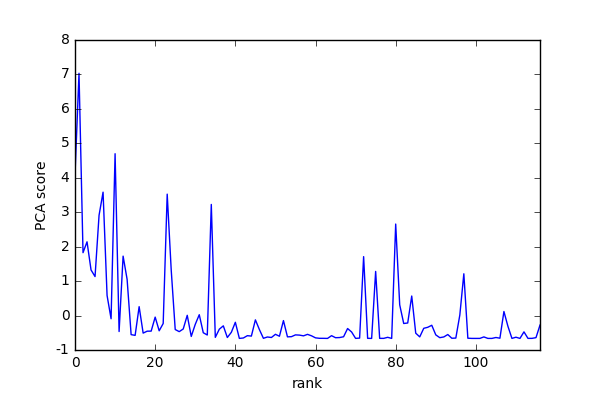
\includegraphics[width=12cm, height=8cm]{graphs/pca.png}
\caption{\label{pca_scores}Principal Component Scores}
\end{figure}

% To do: interpret the results

% √
\subsection{Estimate the Parameters of Utility Function}
In this subsection, the parameters of utility function will be estimated with standard methods of multinomial logit discrete choice model. The parameters are estimated by maximum likelihood estimation, given the assumption of independence of irrelevant alternatives among products. The results are shown in Table \ref{alpha}. The price parameter is negative and the quality parameter is positive, which are consistent with the model predicts. 
\begin{table}[H]
\centering
\begin{tabular}{|c|c|c|c|}
\hline
\textbf{Alpha} & \textbf{Constant} & \textbf{Price} & \textbf{Quality} \\
\hline
\textbf{Value} & -0.02353 & -0.02123 & 0.2639 \\
\hline 
\end{tabular}
\caption{\label{alpha}Demand Parameters}
\end{table}

% TODO: interpretation 

% √
\subsection{Estimate the Marginal Costs of Products}
The final step is to estimate marginal costs of products. Solving the optimization of maximizing profits of seller, we have
$$
(p_{jt}-c_j)D'_{jt}(p_{jt}) + D_{jt}(p_{jt}) = 0
$$
The marginal cost of product $j$ is then:
$$
c_j = p_{jt} + \frac{D_{jt}(p_{jt})}{D'_{jt}(p_{jt})}
$$
 
The demand of product $j$, $D_{jt}(p_{jt})$, is very hard to calculate directly since the count of possible consideration set is too large. Therefore, Monte Carlo methods, which approximate the expectation with respect to a probability distribution, will be used to estimate it and its corresponding derivative. Mathematically, suppose the expectation to be evaluated is 
$$
\mu = \sum_{x}g(x)f(x)
$$
where $x$ is the consideration set, $g(x)= P_{ijt}(x)$ is the individual demand, and $f(x)=\frac{1}{N}x$ is a uniform distribution, where $N$ is the count of all possible consideration set from the given available set. Therefore, an independent Monte Carlo can be summarized is divided into two steps: first, simulate independent draws $t_1$, $t_2$, .... $t_n$ from $f$; second, calculate the estimated expectation:
$$
\hat{\mu}_n = \frac{1}{n} \sum_{i=1}^{n} g(t_i)
$$

Specifically,
$$
\hat{\mu}_n =  \frac{N}{n} \sum_{i=1}^{n} P_{ijt}(x_i)
$$
where $x_1$,... ,$x_i$ , $x_n$ are the sampled consideration sets. 

Practically, it is found that when $n$ is no less than 100, the estimation results are quietly stable. Therefore, the sampling number is selected as 100 in the following estimation and simulation. The estimation results are as Figure \ref{mc}. It can be found that the right side of distribution of marginal costs of sellers is very heavy. This size of distribution is constant with the change of the size of consideration set. 
\begin{figure}[H]
\centering
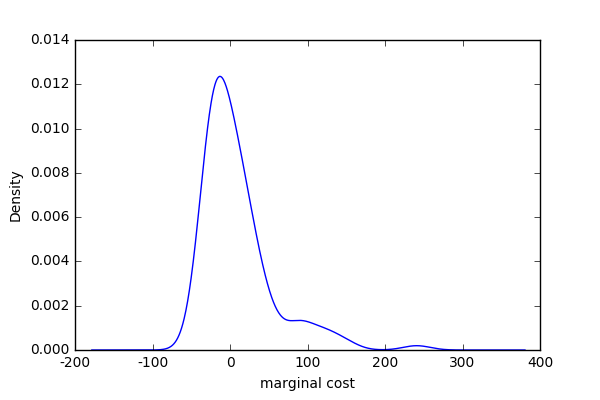
\includegraphics[width=12cm, height=8cm]{graphs/mc.png}
\caption{\label{mc}Marginal Costs of Sellers}
\end{figure}

The summarized statistics of marginal costs are shown in Table \ref{mcstats}. When the size of consideration set is larger than 1/3 of all available products, the summarized statistics of marginal costs of sellers is stable expect the minimum. The mean of marginal costs is around 10, the median is around 0, and the standard deviation is around 45, which is almost the same with the standard deviation of prices. 

\begin{table}[H]
\centering
\begin{tabular}{|c|c|c|c|c|c|c|c|}
\hline
\textbf{Count} & \textbf{Mean} & \textbf{Std} & \textbf{Min} & \textbf{25\%} & \textbf{Median} & \textbf{75\%} &\textbf{Max} \\
\hline
117 & 9.6060 & 45.4375 & -38.5632 & -21.7343 & -1.4238 & 21.2934 & 240.8851 \\
\hline 
\end{tabular}
\caption{\label{mcstats}Summarized Statistics of Marginal Costs}
\end{table}

It has to be noticed that more than half of the estimated marginal costs are negative, which is consistent with the story in the next version of this paper. It is observed in the literatures that sellers tend to seller lower prices to gain higher sales in the beginning periods of entering, and then higher ranks, higher prices and higher sales in the following periods. Therefore, the real pricing of sellers will be much lower than the equilibrium prices assumed in the one-period model, and thus the much lower marginal costs. Therefore, the marginal costs of sellers will be much higher and reliable in the multi-period models, which will be discussed in the next version of this paper. 

% To do: more interpretation

\section{Applications: The Optimal Platform Ranking Algorithm Parameters}

In this version, the estimates will be applied to find the optimal parameters of platform ranking algorithms that maximize the consumer welfare in this market. The algorithm parameters will be allowed to change, and the new optimal parameters will be found under new equilibriums given consumer utility parameters and the marginal costs of sellers. 

Formally, the consumer welfare in this market is 
$$
W = E[u_i] = log(\sum\limits_{j}(exp(u_{ij}))) 
$$

To find the optimal algorithm parameters $\mathbf{\gamma}*$ so that $W(\mathbf{\gamma}*)$ is maximized, the equilibrium prices should be found at first. Given a new $\mathbf{\gamma}'$, the new equilibrium prices can be solved from the Nash equilibrium, that is
$$
\max_{p'_j} (p'_{jt}-c_{j})D_{jt}(p'_{jt}|\mathbf{\gamma}')
$$ 
for each sellers $j$.

Computationally, the new equilibrium prices given new algorithm parameters are solved by fixed-point method. That is, given a initial vector of prices $\mathbf{P}=(p_1, ..., p_n)$, where $n$ is the count of products in the market, the new equilibrium prices for each sellers $1, 2,..., n$ are solved one by one, and a new vector $\mathbf{P^{next}}=(p^{next}_1, ..., p^{next}_n)$ is found. Then the new vector is applied to repeat this process, until it is convergent to a certain vector $\mathbf{P'}$. 

The optimal algorithm parameters are solved as Table \ref{gamma_opt}. Notice that only the scale of algorithms matters. After standardizing the sum of parameters to 1, the sales parameters need to decrease 13\%, the comments parameter need to increase slightly, about 3\% and the parameters of prices need to increase about 10\%. Therefore,  the sales in the weighting should be decrease for a small part, the comments need to increase for a similar small part, and the prices need to increase for a slight percentage. Therefore, the current parameters are very close to the optimal ones, which shows that the platform algorithms may be good enough, considering the limitation of data for this paper. 

\begin{table}[H]
\centering
\begin{tabular}{|c|c|c|c|}
\hline
\textbf{Gamma} & \textbf{Price} & \textbf{Sales (last period)} & \textbf{Comments (last period)}\\ 
\hline
 \textbf{Value($10^{-5}$)} & 0.03469 & 0.1500 & 0.1821 \\  
\hline 
 \textbf{Standardized Value} & 9.458\% & 40.90\% & 49.65\% \\ 
 \hline
\end{tabular}
\caption{\label{gamma_opt}Optimal Algorithm Parameters}
\end{table}


\section{Discussion}
% What done
In this version, a one-period model on platform ranking algorithms, consumer search and choices, sellers pricing and market equilibrium is constructed and the parameters in the model are estimated. The ranking algorithms allocate sampling weights for products, and products with higher sampling weights will be more likely to be ranked to the top. Consumers search products from the consideration set provided by the ranking algorithms, and make the purchase decision in the consideration set. The sellers set their prices to maximize their profits given the ranking algorithms and the mechanism of consumer search and choice. The parameters in the model are estimated with a sample data of a certain day from a single-product market with quality difference. 

% What to do
There are still a lot of limitation in this version. One is about the definition of a single-product market. Due to the limitation of ranking algorithms itself, there may still have part of irreverent products by a certain keyword. One is about the consumer search on a certain ranking. People may search and choose the same product with more detailed keywords, and they can visit similar results from both website from personal computer and APP from mobile phones. Therefore, only a small part of the sales and comments of the products may come from the keywords selected and collected, without known detailed visit search behaviors and statistics. One is about the consideration set approach. Without detailed visit or click data from the platform, it is hard to clearly define a "consideration set" for each consumer, so a simple definition as the top ranks of search result is used in this paper. The probability of being in the consideration set for a certain product can be estimated with more precise machine learning methods, like logistic regression, Lasso, SVR, since the prediction accuracy is more concerned than interpretation to approximate the mechanism of ranking algorithms. 

% What is the next version
In the next version, a multi-period model with dynamic pricing strategy will be built and its parameters will be estimated. In the multi-period situation, the rankings of products will have a large effect on sales and revenue in next periods, which is determined to a great extent by the sales in last periods. The central idea of dynamic pricing strategies is that the sellers will try to set much lower prices in order to promote the sales and comments in this period, so that they can be ranked higher in the next periods and thus higher sales and revenue even if with higher prices. Therefore, the equilibrium prices in each period except the last period will be much lower than that in the one-period model, and thus the estimated marginal costs will be much higher than that in this version. The story will be more complex if it is assumed that some sellers are lack of foresight or want to leave the market. The nearsighted sellers may choose to behavior like sellers in the last period, which just sets high prices to gain more revenue in this period. In this situation, the equilibrium prices will be very lower for some foresighted sellers and higher for some nearsighted sellers. 

% Contribution



\newpage

\nocite{*}
\bibliographystyle{plain}%
\bibliography{ref.bib}




\end{document}

